\documentclass[11pt]{article}
\usepackage[margin=1in]{geometry}
\usepackage{amsmath,amssymb,bm}
\usepackage{graphicx}
\usepackage{booktabs}
\usepackage{xcolor}
\usepackage[numbers,sort&compress]{natbib}
\usepackage{microtype}
\usepackage{caption}
\usepackage{subcaption}
\usepackage{enumitem}
\usepackage{listings}
\usepackage{authblk}
\usepackage{tikz}
\usetikzlibrary{positioning,arrows.meta,fit,backgrounds}
\usepackage[colorlinks=true,linkcolor=blue!60!black,citecolor=blue!60!black,urlcolor=blue!60!black]{hyperref}
\usepackage[capitalise,nameinlink]{cleveref}

\definecolor{codebg}{gray}{0.96}
\lstset{basicstyle=\ttfamily\footnotesize,backgroundcolor=\color{codebg},frame=single,rulecolor=\color{gray!40},
  columns=fullflexible,keepspaces=true,showstringspaces=false,breaklines=true,xleftmargin=2pt,xrightmargin=2pt,
  language=Python,keywordstyle=\color{blue!50!black},commentstyle=\color{gray!70!black},stringstyle=\color{red!45!black}}
\newcommand{\code}[1]{\texttt{#1}}
\newcommand{\dd}{\mathrm{d}}
\newcommand{\Hvap}{\Delta H_\mathrm{vap}}

\title{pGM-JAX: differentiable polarizable Gaussian multipole electrostatics and molecular
dynamics for force-field parameterization}
\author[1]{Zhen Huang}
\affil[1]{Chemical, Applied, and Materials Physics Graduate Program, Departments of Molecular Biology and
Biochemistry, Chemical and Biomolecular Engineering, Materials Science and Engineering, and Biomedical
Engineering, University of California, Irvine, California 92697, United States}
\date{}

\begin{document}
\maketitle

\begin{abstract}
Polarizable force fields are harder to parameterize than fixed-charge ones because every
observable depends on self-consistent induced dipoles. We present pGM-JAX, an implementation of
the polarizable Gaussian multipole (pGM) model in JAX in which energies, forces, induced dipoles
and virials are differentiable functions of the coordinates, the periodic box and every
parameter. The package contains gas-phase and Ewald models for fitting to quantum-chemical
data, and a GPU molecular dynamics engine built on JAX~MD. The engine uses smooth particle-mesh
Ewald for Gaussian charges and dipoles, the induced-dipole solver of Amber's pmemd-pgm, rigid or
flexible molecules and NVE, Langevin NVT and Monte Carlo NPT ensembles. Induced dipoles are
differentiated implicitly, so a derivative of forces or dipoles costs one extra linear solve.
Against Amber, electrostatic energies of a 512-water box agree to $8\times10^{-11}$ relative,
forces to $9\times10^{-7}$~kcal\,mol$^{-1}$\,\AA$^{-1}$ RMS and induced dipoles to
$10^{-10}$~$e$\,\AA. On one GPU the engine runs this box at 130~ns/day, compared with 96~ns/day
for pmemd-pgm's CUDA code, and 4,096 waters at 44~ns/day (pmemd-pgm: 69). Derivatives of
ensemble averages follow from fluctuation formulas with per-frame parameter gradients taken at
the converged dipoles. We use them to fit Lennard-Jones parameters to the density and heat of
vaporization of liquid water and methanol by Gauss--Newton iteration, one simulation per step.
Bonded terms fitted to DFT data make molecules flexible in the same engine. The repository
contains the code, the tests, the data behind every figure and step-by-step workflows for bonded
and van der Waals parameterization.
\end{abstract}

% =====================================================================================
\section{Introduction}

Molecules polarize in response to their environment, and polarizable force fields describe this
explicitly, usually with induced point dipoles~\cite{ponder2010amoeba,ren2003amoebawater}. Point dipoles need
damping at short range~\cite{thole1981} and exclusion rules for bonded pairs. The polarizable
Gaussian multipole (pGM) model replaces point charges and dipoles by Gaussian
distributions~\cite{elking2007gaussian,wang2019pgm1,wei2020pgm}. The interaction between two
Gaussians is finite at any distance, so every pair of atoms interacts, including bonded ones,
and the model has no exclusions and no separate damping function. Permanent dipoles are
defined along covalent bonds, so they follow the molecular geometry without local
frames~\cite{wei2020pgm}. Polarizabilities and Gaussian widths are typed by
element and environment~\cite{wang2019pgm1}; charges and covalent dipoles are fitted to
quantum-chemical electrostatic potentials with PyRESP~\cite{zhao2022pyresp,duan2024pcmresp} and
transfer between molecules~\cite{zhao2023pgmtransfer}. pGM is implemented in Amber's sander and
pmemd, including the stress tensor for constant-pressure
simulation~\cite{wei2022pgmstress,huang2025pgmtuning,case2023ambertools}, and pGM water models have
been refined against liquid properties~\cite{wu2025pgmwater}.

The remaining parameters (Lennard-Jones or other van der Waals terms, and bonded terms for
flexible molecules) are fitted to condensed-phase properties and to quantum-chemical energies
and forces. For a polarizable model this is expensive: each liquid simulation solves for the
induced dipoles at every step, and derivatives of simulated properties with respect to
parameters are rarely available, so parameters are often tuned by hand or by black-box
search~\cite{wu2025pgmwater}. ForceBalance showed that thermodynamic fluctuation formulas give
these derivatives from a single simulation and made systematic optimization of polarizable water
models possible~\cite{wang2014forcebalance,wang2013iamoeba}. Automatic differentiation removes
most of the remaining work: with JAX~\cite{jax2018} or PyTorch, derivatives of any energy function
come for free. JAX~MD~\cite{schoenholz2020jaxmd}, TorchMD~\cite{doerr2021torchmd},
DiffTRe~\cite{thaler2021difftre} and DMFF~\cite{wang2023dmff} use this for differentiable
simulation and force-field development; DMFF includes multipolar polarizable models.

pGM-JAX is a differentiable implementation of pGM itself, meant as the working tool for pGM
parameterization. Its design goals are:
\begin{enumerate}[nosep]
\item \emph{Exactly Amber's model.} The same energy as sander and pmemd-pgm to numerical
precision, so parameters fitted in pGM-JAX can be used in Amber and vice versa.
\item \emph{Parameters are inputs.} Every energy function takes the parameters as an argument,
with user-defined tying of atoms that share a parameter, so gradients with respect to any subset
of parameters come from \code{jax.grad}.
\item \emph{Derivatives through the induction.} First derivatives use the stationarity of the
energy in the induced dipoles; forces, dipoles and higher derivatives are differentiated
implicitly through the dipole solve.
\item \emph{Fast enough to sample liquids.} A GPU MD engine that runs pGM at the speed of Amber's
CUDA code for small and medium boxes, so that a fitting iteration is one short simulation.
\end{enumerate}
This paper describes the model and its implementation (\cref{sec:model,sec:impl}), validation
against Amber (\cref{sec:validation}), performance (\cref{sec:perf}), and two demonstrations:
flexible molecules in MD and fitting of Lennard-Jones parameters to liquid properties
(\cref{sec:demo}). \Cref{sec:workflows} describes the workflows for fitting bonded and van der
Waals parameters.

% =====================================================================================
\section{Model}\label{sec:model}

\paragraph{Electrostatics.}
Atom $i$ carries a Gaussian charge $q_i$, a permanent dipole $\bm p_i$ and an induced dipole
$\bm\mu_i$, all with the Gaussian width of the atom, $R_i$. The permanent dipole is a sum over
covalent bonds, $\bm p_i=\sum_{j\in\mathrm{cov}(i)} c_{ij}\,\hat{\bm r}_{ij}$, with
$\hat{\bm r}_{ij}$ the unit vector from $i$ to $j$ and $c_{ij}$ a fitted strength, so the
permanent dipoles follow the molecular geometry~\cite{wei2020pgm}. Two Gaussians of widths $R_i$
and $R_j$ interact through
\begin{equation}
\phi_{ij}(r)=\frac{\operatorname{erf}(\beta_{ij}r)}{r},\qquad
\beta_{ij}=\bigl[2(R_i^2+R_j^2)\bigr]^{-1/2},
\end{equation}
which is finite at $r=0$. The permanent energy is a sum over \emph{all} pairs,
\begin{equation}
U_\mathrm{perm}=k_e\sum_{i<j}\,(q_i+\bm p_i\cdot\nabla_i)(q_j+\bm p_j\cdot\nabla_j)\,
\phi_{ij}(|\bm r_i-\bm r_j|),
\end{equation}
where $k_e$ is the Coulomb constant and $\nabla_i$ acts on $\bm r_i$. The induced dipoles
minimize
\begin{equation}\label{eq:functional}
U_\mathrm{ind}(\bm\mu)=\tfrac12\,\bm\mu^\mathsf{T}\bm A\,\bm\mu-\bm\mu^\mathsf{T}\bm E,\qquad
\bm A=\bm\alpha^{-1}+\bm T,
\end{equation}
with $\bm\alpha$ the diagonal matrix of isotropic atomic polarizabilities, $\bm E$ the field of
the permanent Gaussian multipoles and $\bm T$ the Gaussian dipole--dipole tensor
($\bm T_{ij}=k_e\nabla_i\nabla_j\phi_{ij}$ for $i\neq j$). At the minimum
$\bm A\bm\mu^*=\bm E$ and $U_\mathrm{ind}^*=-\tfrac12\bm\mu^{*\mathsf T}\bm E$. Because
$\partial U/\partial\bm\mu=0$ at $\bm\mu^*$, first derivatives of the energy with respect to
positions, box or parameters need no derivative of $\bm\mu^*$ (Hellmann--Feynman). Periodic
systems are summed by Ewald methods; the Gaussian widths enter the real-space kernel only.

\paragraph{Van der Waals.} Lennard-Jones in Amber form,
$U_\mathrm{LJ}=\sum\varepsilon_{ij}\bigl[(R^*_{ij}/r)^{12}-2(R^*_{ij}/r)^6\bigr]$ with
$R^*_{ij}=R^*_i+R^*_j$ and $\varepsilon_{ij}=\sqrt{\varepsilon_i\varepsilon_j}$, optionally with
the long-range tail correction. The free parameters are $R^*_i$ and $\sqrt{\varepsilon_i}$ (the
square root keeps the gradient finite at $\varepsilon_i=0$, as for water hydrogens). For rigid
molecules Lennard-Jones acts between molecules only.

\paragraph{Flexible molecules.} Electrostatics already includes every intramolecular pair, so the
valence terms of a flexible pGM molecule only have to carry what the all-pair electrostatics and
the Lennard-Jones between atoms far apart in the bond graph do not:
\begin{equation}\label{eq:intra}
E_\mathrm{intra}=E_\mathrm{bonded}(\bm R)+\sum_{i<j,\;d_{ij}\ge n_\mathrm{LJ}}U^\mathrm{LJ}_{ij}
+s_{14}\sum_{d_{ij}=3}U^\mathrm{LJ}_{ij},
\end{equation}
with $d_{ij}$ the number of bonds between $i$ and $j$, $n_\mathrm{LJ}=4$ by default (Lennard-Jones
from 1--5 pairs on) and an optional scaled 1--4 term. $E_\mathrm{bonded}$ is a sum of term
families (\cref{sec:bonded}) fitted to quantum-chemical energies and forces with exactly this
nonbonded model, so the same energy is used in fitting and in MD.

% =====================================================================================
\section{Implementation}\label{sec:impl}

\Cref{fig:overview} shows the structure of the package. Everything is written in JAX and runs on
CPUs and GPUs; float64 is used throughout except in the MD engine's mixed-precision mode.

\begin{figure}[t]
\centering
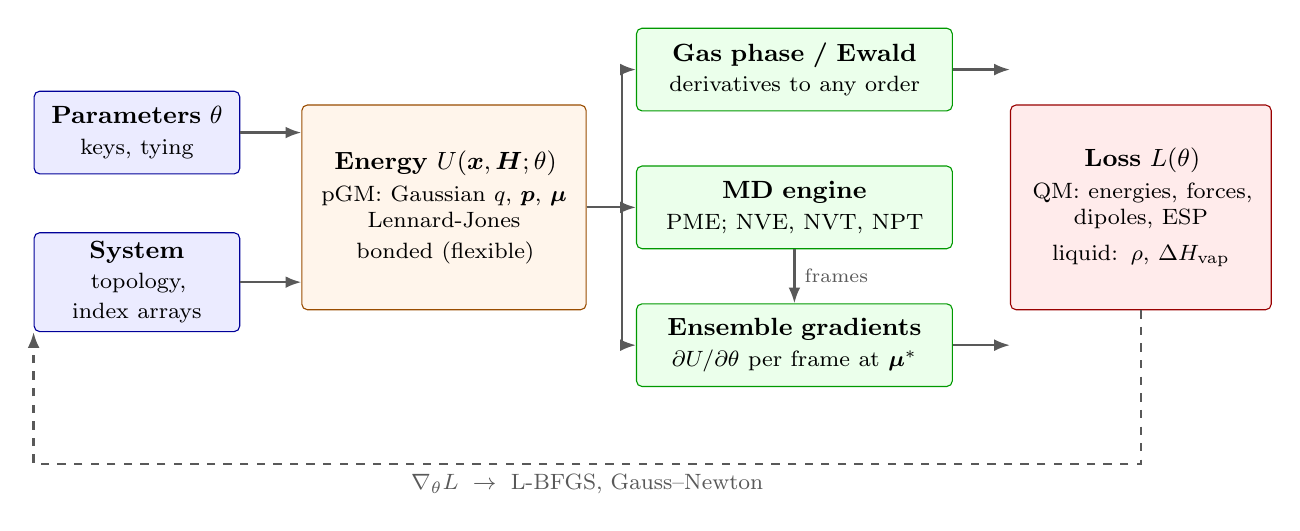
\begin{tikzpicture}[
  box/.style={draw=#1!60!black,fill=#1!8,rounded corners=2pt,align=center,font=\small,
              minimum height=1.05cm,inner sep=3pt},
  arr/.style={-{Latex[length=2mm]},thick,gray!70!black}]
\node[box=blue,text width=2.4cm] (par) at (0,0.95) {\textbf{Parameters $\theta$}\\\footnotesize keys, tying};
\node[box=blue,text width=2.4cm] (sys) at (0,-0.95) {\textbf{System}\\\footnotesize topology, index arrays};
\node[box=orange,text width=3.4cm,minimum height=2.6cm] (en) at (3.9,0) {\textbf{Energy} $U(\bm x,\bm H;\theta)$\\[2pt]\footnotesize
  pGM: Gaussian $q$, $\bm p$, $\bm\mu$\\ Lennard-Jones\\ bonded (flexible)};
\node[box=green,text width=3.8cm] (gas) at (8.35,1.75) {\textbf{Gas phase / Ewald}\\\footnotesize derivatives to any order};
\node[box=green,text width=3.8cm] (md) at (8.35,0) {\textbf{MD engine}\\\footnotesize PME; NVE, NVT, NPT};
\node[box=green,text width=3.8cm] (ens) at (8.35,-1.75) {\textbf{Ensemble gradients}\\\footnotesize $\partial U/\partial\theta$ per frame at $\bm\mu^*$};
\node[box=red,text width=3.1cm,minimum height=2.6cm] (loss) at (12.75,0) {\textbf{Loss} $L(\theta)$\\[2pt]\footnotesize
  QM: energies, forces,\\ dipoles, ESP\\[2pt] liquid: $\rho$, $\Delta H_\mathrm{vap}$};
\draw[arr] (par.east) -- (en.west |- par.east);
\draw[arr] (sys.east) -- (en.west |- sys.east);
\draw[arr] (en.east) -- ++(0.45,0) |- (gas.west);
\draw[arr] (en.east) -- (md.west);
\draw[arr] (en.east) -- ++(0.45,0) |- (ens.west);
\draw[arr] (md.south) -- node[right,font=\scriptsize]{frames} (ens.north);
\draw[arr] (gas.east) -- (loss.west |- gas.east);
\draw[arr] (ens.east) -- (loss.west |- ens.east);
\draw[arr,dashed] (loss.south) -- ++(0,-1.95) -| node[pos=0.25,below,font=\footnotesize]
  {$\nabla_\theta L$ \;$\rightarrow$\; L-BFGS, Gauss--Newton} (par.south west |- sys.south);
\end{tikzpicture}
\caption{Structure of pGM-JAX. Parameters are an explicit input of every energy function;
gradients of a loss with respect to them come from automatic differentiation of the gas-phase or
periodic models, or from fluctuation formulas over MD frames.}
\label{fig:overview}
\end{figure}

\subsection{Parameters as inputs}
A \code{Molecule} holds a topology and initial parameter values (read from an Amber pGM prmtop or
PyRESP output). A \code{ParamTable} turns them into free parameters: for each quantity ($q$,
covalent-dipole strength $c$, width $R$, polarizability $\alpha$, $R^*$, $\sqrt\varepsilon$) a list
of keys, one value per key. Atoms with the same key share one value and one gradient. By default
symmetry-equivalent atoms of a molecule share charges and dipole strengths (as in PyRESP), found
by colour refinement on the bond graph and the covalent-dipole pairs, and $R$, $\alpha$ and the
Lennard-Jones parameters are shared by atom type; any other tying is set by giving keys. One table
built from several molecules ties parameters across them. The parameter pytree is an argument of
every energy function, so \code{jax.grad} returns a pytree of the same shape:

\begin{lstlisting}
sys = System([water] * 3)                      # topology + index arrays into the table
P = sys.table.initial()                        # {"q": ..., "cov": ..., "lj_sqrt_eps": ...}
E = Model([ElecChannel(), LJChannel()]).energy_fn(sys)
dE_dP = jax.grad(lambda p: E(pos, p)["total"])(P)                        # same pytree as P
F = Model([ElecChannel(), LJChannel()]).forces_fn(sys)
dL_dP = jax.grad(lambda p: jnp.sum((F(pos, p) - F_qm) ** 2))(P)          # force matching
\end{lstlisting}

\subsection{Differentiating through the induced dipoles}
In the gas phase the dipoles come from a dense solve of $\bm A\bm\mu=\bm E$ (up to a few thousand
atoms); periodic single-point models use Ewald summation with integer image and $k$-vector lists,
so the box matrix is a differentiable input, and solve by conjugate gradients. The energy is
wrapped so that first derivatives use stationarity and higher derivatives differentiate through
the solve by implicit differentiation~\cite{blondel2022implicit}. Differentiating $\bm A\bm\mu^*=
\bm E(\theta)$ gives $\bm A\,\dd\bm\mu^*=\dd\bm E-\dd\bm A\,\bm\mu^*$, so a vector--Jacobian
product with $\bar{\bm\mu}$ needs one adjoint solve,
\begin{equation}\label{eq:adjoint}
\bm A\bm\lambda=\bar{\bm\mu},\qquad
\bar{\bm\mu}\cdot\frac{\dd\bm\mu^*}{\dd\theta}=\bm\lambda\cdot\frac{\partial(\bm E-\bm A\bm\mu)}{\partial\theta}\Big|_{\bm\mu^*},
\end{equation}
with the same symmetric operator. We checked that this matters: a deliberately broken version that
treats $\bm\mu^*$ as a constant gives second-order parameter derivatives that are wrong by
12--100\,\%, while the implicit version agrees with finite differences
(\cref{sec:validation}).

\subsection{Molecular dynamics engine}\label{sec:md}
The MD engine (\code{pgm\_jax.md}) follows pmemd-pgm~\cite{wei2020pgm,wei2022pgmstress,huang2025pgmtuning}
and uses JAX~MD~\cite{schoenholz2020jaxmd} for cell lists and rigid-body integration.

\emph{Electrostatics.} Smooth PME~\cite{essmann1995spme} for Gaussian charges and total dipoles
($\bm p+\bm\mu$), spread with B-spline derivatives. The real-space part runs over ``rows'': each
atom's intramolecular partners, then its intermolecular neighbours, compacted every step to the
pairs inside the cutoff and stored as a structure of arrays, with per-atom sums and analytic pair
forces instead of scatter-adds. Lennard-Jones uses the same rows, with an optional long-range
tail correction.

\emph{Neighbour lists.} For rigid molecules the list is built between molecular centres with
JAX~MD's cell list; rotations never invalidate it, so for water it is rebuilt about every 30 steps
instead of every 10 for an atom list, at a tenth of the cost. Every overflow of a list or of the
row capacity is detected, the capacities are enlarged and the block of steps is repeated. When the
box volume drifts by more than 10\,\% (NPT from a loose start) or a block keeps overflowing, the
lists are rebuilt for the new box and the block is split.

\emph{Induced dipoles.} As in pmemd-pgm's GPU code: the initial guess is a cubic extrapolation from
the dipoles of the last four steps, the first residual is fused with the permanent-field
evaluation, and a Jacobi-preconditioned conjugate-gradient solve runs to pmemd-pgm's convergence
criterion ($\max|\alpha r|/\operatorname{mean}|\alpha E|\le$ \code{dipole\_scf\_tol}, default
$10^{-5}$), followed by a ``peek'' step. Forces are evaluated at the converged dipoles.

\emph{Integrators.} Rigid molecules are JAX~MD rigid bodies integrated with the NO\_SQUISH
quaternion scheme~\cite{miller2002nosquish}. Flexible molecules are integrated atom by atom with the
bonded energy of \cref{eq:intra}, evaluated for all molecules of a type with one vectorized call,
and are kept whole across periodic boundaries. Temperature is controlled by BAOAB Langevin
dynamics~\cite{leimkuhler2013baoab} with an exact Ornstein--Uhlenbeck step (on centre-of-mass and
body-frame angular momenta for rigid molecules), pressure by an isotropic Monte Carlo
barostat~\cite{chow1995mcbarostat,aqvist2004mcbarostat} with molecular scaling and an adaptive
step. Two issues of JAX~MD 0.2.29 are worked around: its rigid-body Langevin step draws the
quaternion-momentum noise with a diagonal covariance, which leaves water rotations 15--25~K too
cold, and its neighbour list flags valid box matrices as malformed.

\emph{Precision and I/O.} In mixed precision, pair kernels, PME and CG vectors are float32 and
positions, energies and reductions float64; float32 matrix products are requested at full
precision because the default TF32 mode of NVIDIA GPUs made the PME dipole spreading
$10^{-3}$ inaccurate. Any reduced triclinic box is supported. Inputs are Amber prmtop and
inpcrd/rst7 files; trajectories and restarts are Amber NetCDF, and checkpoints continue a run
exactly up to floating-point summation order.

\emph{Differentiable forces and dipoles.} With \code{differentiable=True} the force routine
returns energy, forces and induced dipoles that can be differentiated with respect to parameters,
positions and box, through a custom vector--Jacobian product that implements \cref{eq:adjoint}
with one extra CG solve. The forward pass is unchanged, so MD runs at the same speed with the
option on, and force or dipole matching on periodic frames is a few lines:

\begin{lstlisting}
ff = PGMForceField(system, H, MDSettings(precision="double", differentiable=True))
rows = ff.rows_for(pos, H)                                 # once per frame, on the host
def loss(theta):
    res = ff.compute(pos, H, rows, ff.init_induction(), theta)
    return jnp.sum((res.forces - F_ref) ** 2) + w * jnp.sum((res.induction.mu - mu_ref) ** 2)
g = jax.jit(jax.grad(loss))(system.params0)
\end{lstlisting}

\subsection{Derivatives of ensemble averages}\label{sec:ensemble}
Trajectories themselves are not differentiated: neighbour-list rebuilds, Monte Carlo moves and
the Langevin noise make that neither possible nor useful. For an NPT ensemble at parameters
$\theta$ and an observable $A(\bm x,V;\theta)$,
\begin{equation}\label{eq:fluct}
\frac{\dd\langle A\rangle}{\dd\theta}=\Bigl\langle\frac{\partial A}{\partial\theta}\Bigr\rangle
-\beta\Bigl(\Bigl\langle A\,\frac{\partial U}{\partial\theta}\Bigr\rangle
-\langle A\rangle\Bigl\langle\frac{\partial U}{\partial\theta}\Bigr\rangle\Bigr),
\end{equation}
as used in ForceBalance~\cite{wang2014forcebalance}. The only model-specific quantity is
$\partial U/\partial\theta$ for each saved frame. Because the pGM energy is stationary in the
induced dipoles, it is the partial derivative at fixed converged dipoles, one reverse-mode pass
through the energy (\code{energy\_fixed\_mu}), with no derivative of the dipole solve. For the
density $\rho=M/V$ and the heat of vaporization
$\Hvap=\langle U_\mathrm{gas}\rangle-\langle U_\mathrm{liq}\rangle/N+RT$, \cref{eq:fluct} gives the
Jacobian of both targets with respect to any set of parameters from one liquid simulation. For
molecules without intramolecular Lennard-Jones pairs (rigid molecules, and the flexible methanol
below) $\langle U_\mathrm{gas}\rangle$ does not depend on the Lennard-Jones parameters; otherwise
\cref{eq:fluct} applies to gas-phase frames as well.

\subsection{Bonded terms}\label{sec:bonded}
Because pGM has no exclusions, the bonded terms of a flexible pGM molecule differ from those of
fixed-charge force fields such as GAFF~\cite{wang2004gaff}: they correct an all-pair electrostatic
energy instead of replacing a masked one. \code{pgm\_jax.bonded} provides the topology (internal
coordinates and coupling index sets from the bond graph), a registry of term families (the class~II
set~\cite{dauberosguthorpe2019} used by Abdullah et al.~\cite{abdullah2025bonded}, with Morse bonds, cosine
angles, Fourier torsions and bond--bond, bond--angle, angle--angle, torsion--bond, torsion--angle
and angle--angle--torsion couplings, plus Urey--Bradley and other topological pair terms,
out-of-plane terms and others; a new family is about 20 lines), the model of \cref{eq:intra} with
gas-phase pGM, and an L-BFGS fitter to energies, forces and dipoles. Reference data are frames
sampled with MACE-OFF~\cite{kovacs2025maceoff} and labelled at the
$\omega$B97M-D3(BJ)/def2-TZVPPD level~\cite{mardirossian2016wb97mv,najibi2018wb97md3bj,grimme2011d3bj,rappoport2010def2}
with Psi4~\cite{smith2020psi4}. A study of which functional forms work best with all-pair Gaussian
electrostatics will be reported separately; here the fitted parameters are exported as a
\code{FlexibleTemplate} for the MD engine (\cref{sec:flex}).

% =====================================================================================
\section{Validation}\label{sec:validation}

\Cref{tab:validation} compares pGM-JAX with Amber for a box of 512 rigid three-site pGM waters
with Lennard-Jones on oxygen. Amber's pGM code uses a Coulomb constant
($332.05382$~kcal\,\AA\,mol$^{-1}$\,$e^{-2}$) that is $2.98\times10^{-5}$ smaller than the CODATA
value used by pGM-JAX; comparisons rescale by this ratio.

\begin{table}[t]
\centering\small
\caption{pGM-JAX against Amber for 512 pGM waters: differences unless stated otherwise.
Energies in kcal/mol, forces in kcal\,mol$^{-1}$\,\AA$^{-1}$, dipoles in $e$\,\AA.}
\label{tab:validation}
\begin{tabular}{@{}p{6.2cm}p{8.6cm}@{}}
\toprule
Comparison & Result \\
\midrule
Gas-phase cluster vs sander (no cutoff) & electrostatic energy $2\times10^{-5}$ of $-505{,}230$;
forces $4.2\times10^{-5}$ RMS (RMS force 38.8); LJ 623.8568, identical \\
Periodic vs pmemd-pgm (PME $72^3$, order 8, float64) & electrostatic energy $4\times10^{-5}$ of
$-506{,}165$; forces $8.8\times10^{-7}$ RMS; induced dipoles of every atom $1.2\times10^{-10}$ RMS;
LJ 690.1238, identical \\
Same, MD engine in mixed precision & electrostatic energy 0.05; forces $4\times10^{-4}$ RMS
(RMS force 36); dipoles $8\times10^{-7}$ RMS \\
Molecular virial vs sander ($ntp=1$), no LJ tail & 547.49803 vs 547.498 (values) \\
Same, with LJ tail correction & 610.73566 vs 610.7357 (values) \\
Water monomer vs PyRESP & induced dipoles to $8\times10^{-10}$ a.u. \\
NPT, 298~K, 1~bar (8~\AA\ cutoff, PME $48^3$, order 8, no LJ tail, \code{dipole\_scf\_tol}
$10^{-4}$), 2 runs of 100~ps & density $1.0058\pm0.011$ and $1.0107\pm0.012$ g\,cm$^{-3}$
(pmemd-pgm, same settings: $1.0076\pm0.012$); first peak of $g_\mathrm{OO}$ at 2.79~\AA, height
3.00 (pmemd-pgm: 2.795~\AA, 2.99) \\
\bottomrule
\end{tabular}
\end{table}

Derivatives are tested against finite differences in the test suite (\code{pytest}, 51 tests,
4 minutes on a CPU node): analytic real-space row forces against automatic differentiation
and finite differences ($2\times10^{-10}$ relative in float64); forces and the virial (the
derivative with respect to the box) against finite differences; derivatives of forces and
induced dipoles with respect to parameters, positions and box against finite differences with
the dipoles re-solved ($10^{-7}$ to $10^{-10}$ relative in float64; mixed-precision gradients
agree with float64 to $10^{-6}$ to $5\times10^{-5}$); and second derivatives of the energy with
respect to parameters. Other tests compare PME with exact Ewald sums, check that the neighbour
list is complete in skewed boxes, equipartition between translation and rotation under the
Langevin thermostat, NVE energy conservation, exact restarts and the flexible-molecule engine
(\cref{sec:flex}).

In NVE with mixed precision and a 1~fs step, the energy drift of 512 rigid waters over 20~ps is
$10^{-4}\,kT$/ns per degree of freedom at \code{dipole\_scf\_tol}\,$=10^{-5}$ and 0.02~$kT$/ns at
$10^{-4}$. Under Langevin dynamics ($\gamma=2$~ps$^{-1}$) the temperature is 297--299~K with equal
translational and rotational temperatures.

% =====================================================================================
\section{Performance}\label{sec:perf}

\begin{figure}[t]
\centering
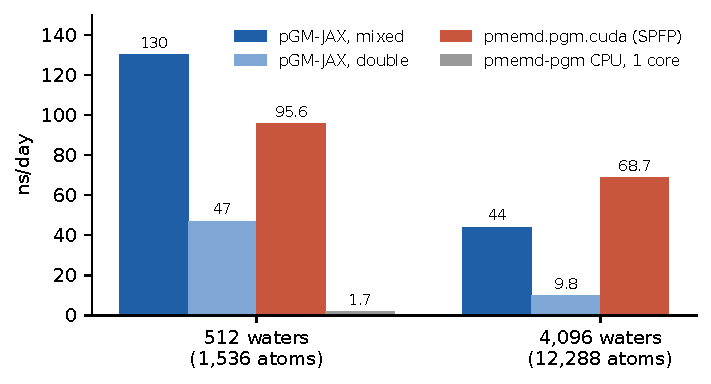
\includegraphics[width=0.78\linewidth]{figures/speed.pdf}
\caption{MD speed on one NVIDIA RTX PRO 6000 Blackwell GPU (pmemd-pgm CPU: one core). NVT,
$\gamma=1$~ps$^{-1}$, 9~\AA\ cutoff, PME grid $48^3$ per 512 waters, order 6, 1~fs step,
\code{dipole\_scf\_tol}\,$=10^{-5}$.}
\label{fig:speed}
\end{figure}

\Cref{fig:speed} compares the MD engine with pmemd-pgm under identical settings. For 512 waters
(1,536 atoms) pGM-JAX runs at 130~ns/day in mixed precision (47 in double), against 95.6~ns/day for
\code{pmemd.pgm.cuda\_SPFP} and 1.7~ns/day for pmemd-pgm on one CPU core. For 4,096 waters (12,288
atoms) it runs at 44~ns/day (9.8 in double) against 68.7. With \code{dipole\_scf\_tol}\,$=10^{-4}$ the
speeds are 148 and 53~ns/day (1.63~ms per step for 12k atoms). The step became fast through the
molecular-centre neighbour list (list cost per step from about 1~ms to 0.03~ms at 12k atoms), row
storage as a structure of arrays (the row kernels are memory bound), a direct PME dipole gradient
inside the CG iteration instead of automatic differentiation, closed-form $3\times3$ box inverses,
and the fused residual. The remaining gap to pmemd-pgm at 12k atoms is hand-written CUDA against
XLA: pmemd-pgm runs one fused kernel per term and CG iteration, XLA several kernels with the loop
condition checked on the host. A gradient of forces and dipoles with respect to all parameters
costs about 15 force evaluations (30~ms for 12k atoms).

% =====================================================================================
\section{Demonstrations}\label{sec:demo}

\subsection{Flexible molecules in MD}\label{sec:flex}
We tested the flexible-molecule engine on liquid methanol. The bonded terms are the class~II set
(Morse bonds, cosine angles, Fourier torsions, an improper term and bond--bond, bond--angle,
angle--angle, torsion--bond, torsion--angle and angle--angle--torsion couplings), fitted with the
all-pair pGM model of \cref{eq:intra} to DFT energies and forces of 224 frames (MACE-OFF
molecular dynamics at 500~K and relaxed torsion scans). On 400 test frames sampled at 298~K they
give an energy error of 0.13~kcal/mol (mean absolute, after removing the mean offset) and a mean
force error of 2.3~kcal\,mol$^{-1}$\,\AA$^{-1}$ per atom. The pGM charges and covalent dipoles come
from PyRESP, the Lennard-Jones parameters from GAFF. Methanol has no pairs more than three bonds
apart, so \cref{eq:intra} contains no Lennard-Jones term here.

\begin{figure}[t]
\centering
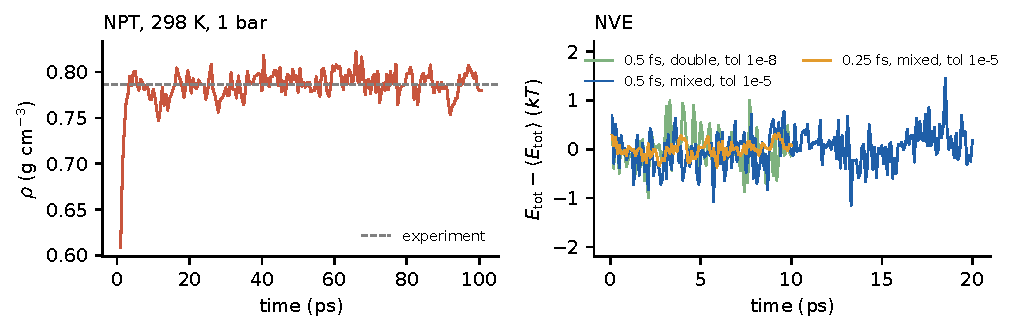
\includegraphics[width=\linewidth]{figures/flexible.pdf}
\caption{216 flexible methanols (1,296 atoms). Left: density under NPT (298~K, 1~bar) from a
dilute start at 0.55~g\,cm$^{-3}$ (GAFF Lennard-Jones); dashed: experiment. Right: total energy in
NVE from the equilibrated state, relative to its mean, in units of $kT$.}
\label{fig:flex}
\end{figure}

\begin{table}[t]
\centering\small
\caption{Checks of flexible-molecule MD for 216 methanols (tol.: \code{dipole\_scf\_tol}; NVE drifts per degree of freedom).}
\label{tab:flex}
\begin{tabular}{@{}p{5.9cm}p{9.9cm}@{}}
\toprule
Check & Result \\
\midrule
One molecule in a 4~nm box vs the gas-phase model (double precision, 1.8~nm cutoff) & max.\ force difference 0.24~kJ\,mol$^{-1}$\,nm$^{-1}$ for an RMS force of 939 ($2.6\times10^{-4}$) \\
NPT, 298~K, 1~bar, 100~ps from 0.55~g\,cm$^{-3}$ & $\rho=0.789\pm0.002$~g\,cm$^{-3}$ over the last 50~ps (standard deviation 0.012; experiment 0.7866); 0.77 reached after 3~ps \\
Temperatures (NPT, last 50~ps) & 296.0~K centre of mass, 295.9~K internal (target 298~K) \\
NVE, 0.5~fs, mixed precision, tol.\ $10^{-5}$, 20~ps & drift $+0.004\,kT$/ns per degree of freedom; RMS fluctuation $0.37\,kT$ (whole system) \\
NVE, 0.25~fs, mixed precision, tol.\ $10^{-5}$, 10~ps & drift $+0.003\,kT$/ns; fluctuation $0.14\,kT$ \\
NVE, 0.5~fs, double precision, tol.\ $10^{-8}$, 10~ps & drift $-0.0005\,kT$/ns; fluctuation $0.40\,kT$ \\
Speed (NPT, Monte Carlo move every 25 steps, one GPU) & 52~ns/day (0.83~ms per step) \\
\bottomrule
\end{tabular}
\end{table}

\Cref{tab:flex} and \cref{fig:flex} summarize the checks. For a single molecule, the forces of the
MD engine (PME electrostatics, bonded terms) agree with the gradient of the gas-phase model the
bonded terms were fitted with, up to the interaction with periodic images and the PME error. A box
started at 0.55~g\,cm$^{-3}$ reaches 0.77~g\,cm$^{-3}$ within 3~ps (the neighbour lists are rebuilt on
the way) and fluctuates around 0.789~g\,cm$^{-3}$ with GAFF Lennard-Jones, against 0.7866 in
experiment~\cite{srivastava1987methanol}. Translational and internal temperatures agree, so the
Langevin thermostat equilibrates the fast bond vibrations and the molecular motion alike. In NVE
the total energy is conserved: the drift is below $0.005\,kT$/ns per degree of freedom in all three runs, which is the precision of these 10--20~ps estimates; the fluctuation drops from 0.37 to $0.14\,kT$ when the time step is halved, and double precision with a $10^{-8}$ dipole tolerance does not change it, so the remaining error comes from the integrator, not from the induction solver. At 0.5~fs the engine runs 52~ns/day for this
system.

\subsection{Lennard-Jones parameters from liquid properties}\label{sec:liquid}
We fitted Lennard-Jones parameters to the density $\rho$ and the heat of vaporization $\Hvap$ at
298~K and 1~bar with \code{scripts/fit\_liquid.py}. The parameters are two global scales,
$\theta=(\ln s_R,\ln s_\varepsilon)$, with $R^*_i\to s_R R^*_i$ and $\varepsilon_i\to s_\varepsilon
\varepsilon_i$ for every atom. Each iteration is one NPT simulation (0.9~nm cutoff with the
Lennard-Jones tail correction, PME spacing 0.08~nm and order 6, \code{dipole\_scf\_tol}\,$=10^{-5}$,
mixed precision, Langevin $\gamma=1$~ps$^{-1}$, Monte Carlo volume moves every 25 steps): 20~ps of
equilibration (100~ps in the first iteration), then 200~ps of production with a frame every
0.2~ps. For each of the 1,000 frames the script evaluates $U$, $V$ and $\partial U/\partial\theta$
at the converged dipoles; \cref{eq:fluct} gives the Jacobian $\bm J$ of $(\rho,\Hvap)$, and the
Gauss--Newton step $\Delta\theta=-(\tilde{\bm J}^\mathsf{T}\tilde{\bm J}+10^{-3}\bm I)^{-1}
\tilde{\bm J}^\mathsf{T}\tilde{\bm r}$, with residuals and Jacobian scaled by 0.005~g\,cm$^{-3}$ and
0.05~kcal/mol, is clipped to $|\Delta\ln s_R|\le0.02$ and $|\Delta\ln s_\varepsilon|\le0.25$. The
next simulation starts from the last configuration and tests the linear prediction
$\bm y+\bm J\Delta\theta$. Standard errors are from five blocks. As a check that the per-frame
derivatives belong to the sampled energy, the energy recomputed from the parameters at every frame
equals the integrator's potential energy to 0.03~kJ/mol for water and 0.01~kJ/mol for methanol
(of totals of $-2\times10^{6}$ and $-1.7\times10^5$~kJ/mol).

\begin{figure}[t]
\centering
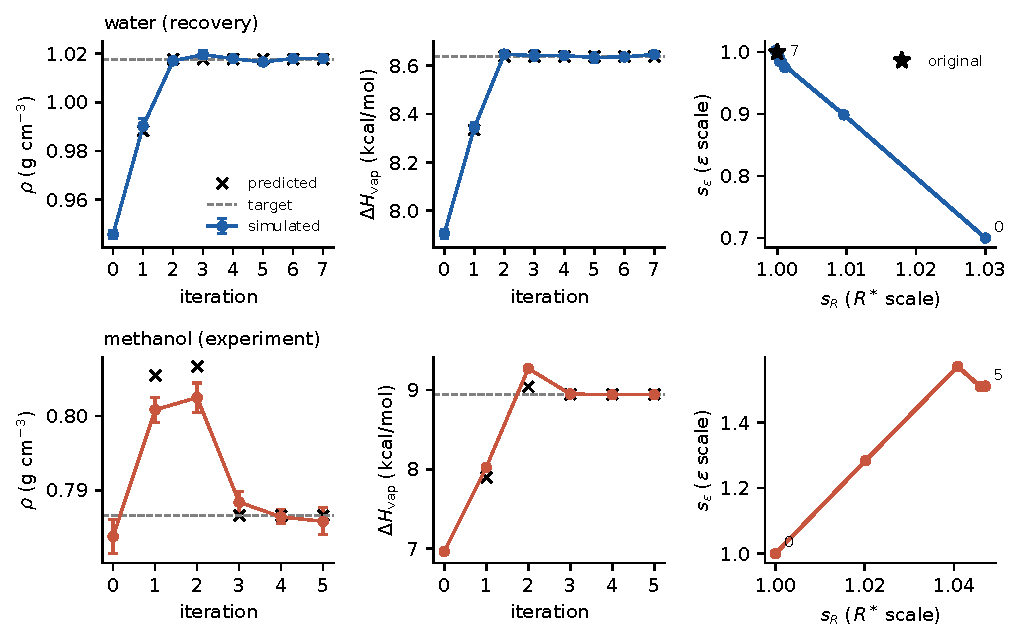
\includegraphics[width=\linewidth]{figures/liquid_fit.pdf}
\caption{Gauss--Newton fits of two Lennard-Jones scales to the liquid density and heat of
vaporization. Top: parameter recovery for 512 rigid pGM waters, from $s_R=1.03$,
$s_\varepsilon=0.70$ to the model's own properties at $s_R=s_\varepsilon=1$. Bottom: 216 flexible
methanols from GAFF Lennard-Jones to experiment. Circles: simulated averages ($\pm2$ standard
errors); crosses: values predicted from the previous iteration's Jacobian; dashed: targets.
Right: path of the parameters.}
\label{fig:liquid}
\end{figure}

\paragraph{Water: parameter recovery.}
For 512 rigid pGM waters (1~fs time step) the targets were the model's own values at its original
parameters from a 400~ps run, $\rho=1.0177\pm0.0009$~g\,cm$^{-3}$ and
$\Hvap=8.638\pm0.008$~kcal/mol ($U_\mathrm{gas}$ is the exact energy of the rigid monomer). Starting from $s_R=1.03$ and $s_\varepsilon=0.70$ ($\rho=0.946$, $\Hvap=7.905$), the
fit reached the targets within their statistical errors in two iterations (\cref{fig:liquid},
top): the second iteration predicted $(1.0177,\,8.638)$ and gave
$(1.0171\pm0.0003,\,8.647\pm0.007)$. Over iterations 2--7 the parameters stayed at
$s_R=1.0005\pm0.0005$ and $s_\varepsilon=0.985\pm0.009$ (mean and standard deviation), consistent
with the original values and with the precision expected from the Jacobian and the standard
errors (0.0006 in $\ln s_R$ and 0.014 in $\ln s_\varepsilon$, correlation $-0.99$). The two targets
constrain $\varepsilon$ only weakly for water: both respond to $\varepsilon$ through nearly the same
combination as to $R^*$ (the scaled Jacobian has condition number 170), and both derivatives with
respect to $\ln s_\varepsilon$ are negative ($\partial\rho/\partial\ln s_\varepsilon=-0.13$~g\,cm$^{-3}$,
$\partial\Hvap/\partial\ln s_\varepsilon=-2.7$~kcal/mol) because the Lennard-Jones energy of liquid
water is repulsive overall ($+690$~kcal/mol for the 512-water configuration of
\cref{tab:validation}). An iteration took 200~s on one GPU. The
original parameters of this model give a heat of vaporization 1.9~kcal/mol below experiment
(10.52~kcal/mol~\cite{horn2004tip4pew}) at a density 2\,\% above experiment. A linear
extrapolation from the Jacobian puts both experimental values at $s_R\approx1.08$ and
$s_\varepsilon\approx0.08$, far outside the range where two global Lennard-Jones scales are a
sensible model, so a fit of this water model to experiment needs other parameters (charges,
polarizabilities or the form of the repulsion) to move as well.

\paragraph{Methanol: fit to experiment.}
For 216 flexible methanols (0.5~fs time step; bonded terms of \cref{sec:flex}) the targets were
the experimental $\rho=0.7866$~g\,cm$^{-3}$~\cite{srivastava1987methanol} and
$\Hvap=37.43$~kJ/mol $=8.946$~kcal/mol~\cite{polak1971hvap}. $\langle U_\mathrm{gas}\rangle$ comes from
gas-phase Langevin dynamics with the same bonded and pGM model (16 replicas of 100~ps,
$\pm0.09$~kJ/mol), shifted by the difference between the MD engine and the gas-phase model for one
molecule in a large box. With GAFF Lennard-Jones parameters the model gives
$\rho=0.7838\pm0.0011$~g\,cm$^{-3}$, close to experiment, but $\Hvap=6.965\pm0.014$~kcal/mol, 2~kcal/mol
too low. Here $\varepsilon$ is well determined: $\partial\Hvap/\partial\ln s_\varepsilon=+4.4$ to
$+7.4$~kcal/mol, positive because in liquid methanol the Lennard-Jones energy is attractive overall
($-2.5\times10^3$~kJ/mol for 216 molecules). The fit reached both targets in four iterations (\cref{fig:liquid}, bottom). At $s_R=1.047$ and
$s_\varepsilon=1.510$ the fourth iteration gave $\rho=0.7864\pm0.0005$~g\,cm$^{-3}$ and
$\Hvap=8.941\pm0.010$~kcal/mol, and the fifth, after a step below $10^{-3}$, $0.7858\pm0.0009$ and
$8.941\pm0.011$. The first two steps were large ($\Delta\ln s_\varepsilon=0.25$ and 0.20, with
$\Delta\ln s_R$ at its limit of 0.02), and their linear predictions missed by 0.004--0.005~g\,cm$^{-3}$ in density and 0.13--0.23
kcal/mol in $\Hvap$; once the steps were small, predictions and simulations agreed within
0.002~g\,cm$^{-3}$ and 0.005~kcal/mol, comparable to the statistical errors of the two simulations
involved. Unlike for water, the Jacobian is well conditioned (condition number 2.4), and the
standard errors translate into uncertainties of 0.06\,\% in $s_R$ and 0.16\,\% in $s_\varepsilon$.
The fit raises the GAFF well depths by 51\,\% and the radii by 4.7\,\%: GAFF Lennard-Jones,
developed for fixed charges, underbinds liquid methanol by 2~kcal/mol when combined with pGM
electrostatics fitted to gas-phase potentials. This is the kind of van der Waals
parameterization that \cref{sec:workflows} is meant for. An iteration took 8--14~min on one GPU
(23~min for the first, which includes 100~ps of equilibration).

% =====================================================================================
\section{Parameterization workflows}\label{sec:workflows}
The repository contains two step-by-step guides (\code{docs/howto\_bonded.md} and
\code{docs/howto\_vdw.md}) and example scripts for the two parameterization tasks that come next in
the pGM effort: bonded terms for flexible molecules, and van der Waals parameters.

\paragraph{Bonded terms (bonds, angles, torsions, couplings).}
\begin{enumerate}[nosep,leftmargin=*]
\item \emph{Reference data.} Topology and conformers from a SMILES string (RDKit); the MACE-OFF
minimum; Langevin MD with MACE-OFF at 500~K (training) and 298~K (test) and relaxed torsion scans;
DFT energies, forces and dipoles for the sampled frames (Slurm arrays; only missing frames are
resubmitted); pGM charges and covalent dipoles fitted to the B3LYP/aug-cc-pVTZ electrostatic
potential with PyRESP and polarizabilities and widths from the pGM table, following the standard
pGM protocol~\cite{wang2019pgm1,zhao2022pyresp}; Lennard-Jones from GAFF~\cite{wang2004gaff} as a
start.
\item \emph{Fit.} \code{python examples/fit\_bonded\_template.py <name> --families paper} fits the
chosen families with the all-pair pGM model of \cref{eq:intra}, reports energy and force errors
on the 298~K frames, and writes a \code{FlexibleTemplate}. Term families are a registry; a new one is
a JAX function of internal coordinates, and the test suite checks its derivatives automatically.
\item \emph{Check in MD.} \code{examples/run\_flexible\_liquid.py} builds a box and runs NVT and NPT;
the checks of \cref{sec:flex} (forces against the gas-phase model, NVE conservation, internal
temperature, density) apply to every new template.
\end{enumerate}

\paragraph{Van der Waals parameters.}
\begin{enumerate}[nosep,leftmargin=*]
\item \emph{Liquid properties.} \code{scripts/fit\_liquid.py} implements \cref{sec:liquid}. The map
from the optimization variables to the parameter table (a \code{ParameterSpace}, built by \code{lj\_space}) is the only place that
decides what is fitted: two global scales in the demonstration, or one $R^*$ and one $\varepsilon$
scale per atom type (\code{--params type}; with more parameters than targets the Gauss--Newton step
is the minimum-norm step, so more targets or a prior are needed). Because $\partial U/\partial\theta$ comes from \code{jax.value\_and\_grad}
through that map, changing the parameterization needs no new derivative code. Further targets
(other temperatures, other liquids, fluctuation properties) add rows to the Jacobian.
\item \emph{Gas-phase data.} Dimer and cluster energies, or SAPT-like electrostatic and induction
components (\code{elec\_decomposition}), are fitted with the gas-phase model and
\code{jax.grad}; a combined objective is the sum of the gas-phase loss and the liquid residuals.
\item \emph{Checks.} The predicted-versus-simulated comparison of each iteration, longer runs with
the final parameters, and the tests of the MD engine.
\end{enumerate}


% =====================================================================================
\section{Limitations and outlook}
The MD engine implements Lennard-Jones only; other van der Waals forms (for example repulsion
from overlapping Gaussian densities) need their own energy channel, real-space kernels and tail
corrections. Flexible molecules have no bond constraints yet, so the time step is 0.5~fs, and
bonded terms can be exported to MD only if they were fitted with the engine's nonbonded model
(pGM with all pairs, no charge flux). The ensemble gradient of $\langle U_\mathrm{gas}\rangle$ is not
yet implemented for molecules with intramolecular Lennard-Jones pairs. For boxes of about
$10^4$ atoms and more, pmemd-pgm's hand-written CUDA kernels remain faster (69 against 44~ns/day for
12k atoms), and pGM-JAX runs on a single GPU. Trajectories are not differentiated; derivatives of
ensemble averages carry the statistical error of the simulation. Fitted parameters are stored as
JSON; writing them into Amber prmtop files is not implemented yet.

Natural next steps are per-type Lennard-Jones fits over several liquids at once, with gas-phase
dimer data as a second objective; derivatives of hydration and solvation free energies, which
need the same per-frame $\partial U/\partial\theta$ within free-energy estimators; and bonded
parameters for the pGM small-molecule library, run through the same MD engine.


\section*{Code availability}
pGM-JAX is available at \texttt{[repository URL]} under \texttt{[license]}. The repository
contains the tests, the Amber validation inputs, the benchmark scripts, the fitting scripts and
the data behind every figure of this paper (\texttt{paper/}).

\section*{Acknowledgments}
[To be added.]

\bibliographystyle{unsrtnat}
\bibliography{references}

\end{document}
